%!TEX option = -enable-write18

\documentclass[9pt,xcolor={svgnames, x11names}]{beamer}

% the following two commands 'seem' to do the same thing...?
% \usefonttheme[onlymath]{serif}
\usefonttheme{professionalfonts}

% \usepackage{amsmath} % not needed as this is automatically loaded by Beamer

\definecolor{staticsstructurecolor}{rgb}{0.45,0,0}
% \usepackage{hyperref} % hyperref usually loaded last but automatically be Beamer
\hypersetup{
  colorlinks,
  citecolor=red,
  filecolor=orange,
  linkcolor=staticsstructurecolor, % table of contents
  urlcolor=staticsstructurecolor
}
% \usepackage{enumitem} % incompatible with Beamer?
\everymath{\displaystyle}

\usepackage[absolute,overlay]{textpos}
\setlength{\TPHorizModule}{1.0cm}
\setlength{\TPVertModule}{\TPHorizModule}
\textblockorigin{0.0cm}{0.0cm}  %start all at upper left corner


%\usepackage{amssymb}
\usepackage{verbatim} % for latex code in latex doc
% \usepackage{shellesc}

\usepackage{tikz}
\usepackage{pgfmath}
% \usepackage{fp}
\tikzset{every picture/.append style={line cap=round}}
\def\scale{1} % initialisation for pikz
\usetikzlibrary{calc} % only works within a path
% \usetikzlibrary{fpu}
\usetikzlibrary{math} % if then else etc.
\usetikzlibrary{arrows.meta}


\usetheme{Antibes}
\usecolortheme[named=staticsstructurecolor]{structure}
% \setbeamertemplate{items}[triangle]
\setbeamertemplate{blocks}[rounded][shadow=false]
\setbeamertemplate{headline}{\vspace{.1cm}}
\setbeamertemplate{navigation symbols}{} % empty braces suppresses all navigation symbols
\setbeamertemplate{footline}{
  \hfill
  \insertshorttitle
  \quad
  \insertsection
  \quad
  \insertsubsection
  \quad
  \insertframenumber/\inserttotalframenumber
  \quad{ }
  \vspace{0.125cm}
}
\addtobeamertemplate{footline}{\hypersetup{linkcolor=black}}{}
\setbeamertemplate{navigation symbols}{} % empty braces suppresses all navigation symbols
\setbeamercolor{frametitle}{fg=white}


% counter for resuming enumerated list numbers
\newcounter{resumeenumi}
\newcommand{\suspend}{\setcounter{resumeenumi}{\theenumi}}
\newcommand{\resume}{\setcounter{enumi}{\theresumeenumi}}

\newcommand\lb{\linebreak}
\newcommand\pars{\par\smallskip}
\newcommand\parm{\par\medskip}
\newcommand\parb{\par\bigskip}

%left flushed minipage
\newcommand{\minit}[2][0.8]{
	\begin{minipage}[t]{#1\columnwidth}
		\raggedright
		#2
	\end{minipage}
}

%left flushed minipage
\newcommand{\mini}[2][0.8]{
	\begin{minipage}[c]{#1\columnwidth}
		\raggedright
		#2
	\end{minipage}
}



% centered minipage with text \raggedright
%\cmini[width]{content}
\newcommand{\cmini}[2][0.8]{
	\begin{center}
		\begin{minipage}{#1\columnwidth}
			\raggedright
			#2
		\end{minipage}
	\end{center}
}

% get x and y coordinates from a tikz coordinate
%\gettikzxy{A}{\ax}{\ay}
\makeatletter
\providecommand{\gettikzxy}[3]{%
	\tikz@scan@one@point\pgfutil@firstofone#1\relax
	\edef#2{\the\pgf@x}%
	\edef#3{\the\pgf@y}%
}
\makeatother

\definecolor{saitMaroon}{RGB}{172, 31, 45}
\definecolor{mucus}{rgb}{0.55,0.53,0.31} 
\definecolor{myGreen}{RGB}{0,150,0}
\definecolor{saitPurple}{RGB}{112,40,119}
\definecolor{saitDeepBlue}{RGB}{0, 99, 167}



%  \definecolor{saitRed}{RGB}{224,38,37} 
%  \definecolor{saitBlue}{rgb}{0, 0.59, 0.85}
%  \definecolor{khaki}{RGB}{190, 183, 107}
 %\definecolor{philpotBlue}{RGB}{13,69,120}
% \definecolor{dRed}{rgb}{0.7,0,0}
% \definecolor{blueGrey}{rgb}{0.4,0.48,0.53}
% \definecolor{white}{rgb}{1,1,1}
% \definecolor{dkgreen}{rgb}{0,0.5,0}
% \definecolor{greenyellow}{rgb}{0.9,0.9,0.5}
% \definecolor{flesh}{rgb}{1, 0.95, 0.8}
% \definecolor{wheat}{rgb}{.96, .87, .70}
% \definecolor{oldlace}{rgb}{.992, .96187, .902}
% \definecolor{snow}{rgb}{1, .98, .98}
% \definecolor{ghostwhite}{rgb}{.973, .973, 1}
% \definecolor{cornsilk}{rgb}{1, .973, .863}
% \definecolor{honeydew}{rgb}{.941, 1, .941}
% \definecolor{lavenderdark}{rgb}{.8, .8, .9529411}
% \definecolor{lavender}{rgb}{.902, .902, .980}
% \definecolor{lightblue}{rgb}{.8, .8, .95}
\definecolor{lightgray}{rgb}{.827, .827, .827}
% \definecolor{lightsteelblue}{rgb}{.690, .769, .871}
% \definecolor{lightturquoise}{rgb}{.686, .933, .933}
% \definecolor{darkgreen}{rgb}{.0, .392, .0}
% \definecolor{yellowgreen}{rgb}{.604, .804, .196}
% \definecolor{vlightblue}{rgb}{.88, .85, .95}
% \definecolor{khaki}{rgb}{.741, .718, .42}
% \definecolor{lightkhaki}{rgb}{1, .96, .7}
% \definecolor{almostwhite}{rgb}{1,.95,1}
% \definecolor{facegreen}{rgb}{.45, .5, .2}
% \definecolor{llllBlueGrey}{rgb}{0.8,0.96,1}
% \definecolor{lllBlueGrey}{rgb}{0.69,0.83,0.92}
% \definecolor{llBlueGrey}{rgb}{0.58,0.69,0.76}
% \definecolor{lBlueGrey}{rgb}{0.48,0.58,0.64}
% \definecolor{blueGrey}{rgb}{0.4,0.48,0.53}
% \definecolor{dBlueGrey}{rgb}{0.33,0.4,0.44}
% \definecolor{ddBlueGrey}{rgb}{0.28,0.33,0.37}
% \definecolor{dddBlueGrey}{rgb}{0.23,0.28,0.31}
% \definecolor{almostBlue}{rgb}{0.985,0.985,1}
% \definecolor{almostGreen}{rgb}{0.9,0.97,0.9}

% \definecolor{almostRed}{rgb}{0.95,0.875,0.8}
%  \definecolor{headerGrey}{RGB}{128,128,128}
%  \definecolor{headerGray}{RGB}{128,128,128}
% \definecolor{dHeaderGrey}{RGB}{96,96,96}
% \definecolor{ddHeaderGrey}{RGB}{64,64,64}
% \definecolor{dddHeaderGrey}{RGB}{32,32,32}
% \definecolor{lHeaderGrey}{RGB}{160,160,160}
% \definecolor{llHeaderGrey}{RGB}{192,192,192}
% \definecolor{lllHeaderGrey}{RGB}{224,224,224}
% \definecolor{philpotBlue}{RGB}{13,69,120}
% \definecolor{drabGreen}{RGB}{156,143,87}
% \definecolor{ground}{RGB}{153,153,51}
% \definecolor{gridLight}{rgb}{0.85,0.85,0.85}
% \definecolor{darkGreen}{rgb}{0,0.5,0}

% !TEX root = ../../statikz/statikz.tex

% get x and y coordinates from a tikz coordinate, returned values in points
\makeatletter
\providecommand{\gettikzxy}[3]{%
  \tikz@scan@one@point\pgfutil@firstofone#1\relax
  \edef#2{\the\pgf@x}%
  \edef#3{\the\pgf@y}%
}
\makeatother

%\Member{startpt}{endpt}{outer}{inner}{stroke}{height}{radius}{line width}
\providecommand{\Member}[8]{
  % name the points
  \coordinate(start) at (#1);
  \coordinate(end) at (#2);
  \def\outer{#3}
  \def\inner{#4}
  \def\stroke{#5}
  \def\hi{#6} % cm
  \def\rad{#7} % cm
  \def\line{#8} % mm

  \def\tocm{0.035146}
  % \def\topt{28.45274}

  \coordinate(delta) at ($ (end)-(start) $);
  \gettikzxy{(delta)}{\dx}{\dy}
  \gettikzxy{(start)}{\sx}{\sy}
  \pgfmathparse{veclen(\dx, \dy)}% \pgfmathresult
  \let\length\pgfmathresult

  \pgfmathparse{\dx==0}%
  % \ifnum low-level TeX for integers
  \ifnum\pgfmathresult=1 % \dx == 0
    \pgfmathsetmacro{\rot}{\dy > 0 ? 90 : -90}
  \else
    \pgfmathsetmacro{\rot}{\dx > 0 ? atan(\dy / \dx) : 180 + atan(\dy / \dx)}
  \fi

  % \begin{scope}[scale=\scale]    
  
    \begin{scope}	[rounded corners = \rad cm, transform canvas = { rotate around = {\rot:(\sx,\sy)}}]
      \shadedraw[top color = \outer, bottom color = \outer, middle color = \inner, draw = \stroke, line width = \line mm] ($ (start)+(-0.5*\hi, 0.5*\hi) $) -- ++(\hi cm +\length pt, 0 ) -- ++(0, -\hi) -- ++ (-\hi cm -\length pt, 0) -- cycle;
    \end{scope}
    \shadedraw[ball color = \outer!50!\inner, draw = \stroke] (start) circle (\hi/8);
    \shadedraw[ball color = \outer!50!\inner, draw = \stroke] (end) circle (\hi/8);

% \end{scope}


}

\newcommand{\Rocker}[6][0]{
	\def\lrotate{#1};
	\def\lpin{#2}
	\def\lfill{#3}
	\def\ldraw{#4}
	\def\lscale{#5}
	\def\lwidth{#6}
	\def\h{1}
	\def\r{0.3}
	\begin{scope}[scale=\lscale, rotate=\lrotate]
        
        \filldraw[draw=\ldraw, fill=\lfill, line width = \lwidth mm] ($(\lpin) + (0,-\h)$)arc(-90:-57.54:\h) -- 
		++(105:0.95394)arc(15:165:\r) -- ++(-105:0.95394)arc(-122.458:-90:\h);

		\shadedraw[ball color=\lfill, draw=\ldraw, line width = \lwidth mm] (\lpin) circle (1.5mm);
		
	\end{scope}
}



%\Rone[rotate=0]{coordinate}{draw}{fill}{scale}{line width}
\newcommand{\RollerOne}[6][0]{
	\def\rotate{#1};
	\def\pin{#2}
	\def\lfill{#3}
	\def\ldraw{#4}
	\def\lscale{#5}
	\def\lwidth{#6}
	\def\h{1}
	\def\r{0.3}

	\begin{scope}[scale=\lscale, rotate=\rotate, line width=\lwidth mm]

		\shadedraw[ball color=\lfill!50, draw=\ldraw] ($ (\pin) + (0,-0.6*\h)$) circle (\h*4 mm);
		\filldraw[rounded corners=2pt, draw=\ldraw, fill=\lfill] ($(\pin) + (-0.52494*\h,-.8*\h)$) -- ++(1.05*\h, 0) -- ++(105:0.9059)arc(15:165:\r) -- cycle;
		\shadedraw[ball color=\lfill, draw=\ldraw, line width=2*\lwidth pt] (\pin) circle (\lscale mm);
		\shadedraw[ball color=\lfill, draw=\ldraw, line width=\lwidth pt] ($ (\pin) + (0,-0.6*\h)$) circle (\h*0.5 mm);



	\end{scope}
}



%\Roller[rotate=0]{coordinate}{draw}{fill}{scale}{line width}
\newcommand{\RollerThree}[6][0]{
	\def\rotate{#1};
	\def\pin{#2}
	\def\lfill{#3}
	\def\ldraw{#4}
	\def\lscale{#5};
	\def\lwidth{#6};
	\def\h{1}
	\def\r{0.3}
	\def\rr{0.15}
	\begin{scope}[scale=\lscale, rotate=\rotate, myshade/.style={outer color = \lfill!70!\ldraw, inner color=\lfill!25!white, draw=\ldraw!90!black, line width=\lwidth mm}]
		
		\shadedraw[myshade] ($(\pin) + (0,-\h+\rr)$) circle (\rr);
		\filldraw[\ldraw!50!black]($(\pin) + (0,-\h+\rr)$) circle (0.5mm);

		\shadedraw[myshade] ($(\pin) + (-0.325,-\h+\rr)$) circle (\rr);
		\filldraw[\ldraw!50!black]($(\pin) + (-0.325,-\h+\rr)$) circle (0.5mm);

		\shadedraw[myshade] ($(\pin) + (0.325,-\h+\rr)$) circle (\rr);
		\filldraw[\ldraw!50!black]($(\pin) + (0.325,-\h+\rr)$) circle (0.5mm);

		\filldraw[rounded corners= \lscale pt, draw=\ldraw, fill=\lfill, line width=\lwidth mm] ($(\pin) + (-0.52494*\h,-.8*\h)$) -- ++(1.05*\h, 0) -- ++(105:0.9059)arc(15:165:\r) -- cycle;

		\shadedraw[ball color=\lfill, \ldraw, line width=\lwidth mm] (\pin) circle (1.5mm);
		\filldraw[rounded corners=\lscale pt, draw=\ldraw, fill=\lfill, line width=\lwidth mm] ($ (\pin) - (0.55*\h,0.825*\h) $) rectangle +(1.1*\h,0.2*\h);
	\end{scope}
}

\input{../pikz/components/RollerOnly}
\input{../pikz/components/PinnedConnection}
\input{../pikz/components/EyeConnection}
\input{../pikz/components/EyeConnectionB}


% various hacks to get around (apparent?) Beamer titlepage constraints
\title[\color{black} Statikz\textcolor{Maroon}{2020}]{\Huge Statikz}
\subtitle{} % i.e., a blank line
\institute{\small Source code at: {\footnotesize\url{https://github.com/dmorgorg/nuLaTeX/blob/master/statikz2020/statikz.pdf}}}
\author{} % another blanky
\date{\small Last updated on \today}

\begin{document} %%%%%%%%%%%%%%%%%%%%%%%%%%%%%%%%%%%%%%%%%%%%%%%%%%%%%%%%%%%%%%%%%%%%%%%%%%%%%%%%%%

\begin{frame}[plain]
  \titlepage
\end{frame}

\begin{frame}{Table of Contents}
  \begin{minipage}{0.9\textwidth}
    \tableofcontents
  \end{minipage}
  \vfill
\end{frame}

\section{Tikz Components} %%%%%%%%%%%%%%%%%%%%%%%%%%%%%%%%%% Components %%%%%%%%%%%%%%%%%%%%%%%%%%%%%%%%
\centering

%%%%%%%%%%%%%%%%%%%%%%%%%%%%%%%%%%%%%%%%%%%%%%%%%%%%%%%%%%%%%%%%%%%%%%%%%%%%%%%%%%%%%%%%%%%%%%%%%%%
% Note that use of verbatim within Beamer needs fragile setting for frame
% Also, verbatim environment cannot be inside curly braces, {\begin{verbatim}... blows up?
\begin{frame}[fragile]{Tikz Components :: Member}

  \small
  \begin{verbatim}
     \Member{startpt}{endpt}{outer}{inner}{stroke}{height}{radius}{line width}
   \end{verbatim}
  \parb
 
  % \resizebox{0.25\textwidth}{!}{%
  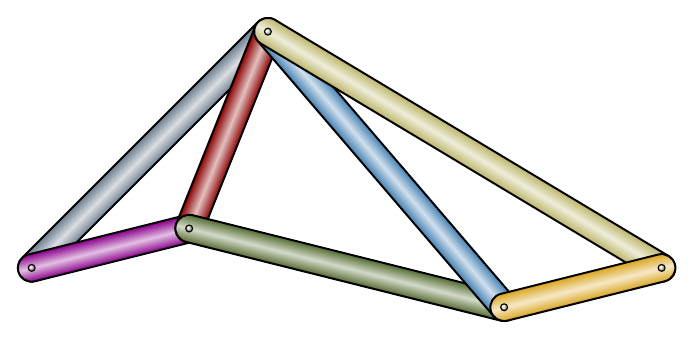
\begin{tikzpicture}
    \coordinate (A) at (0,0);
    \coordinate (B) at (3,3);
    \coordinate (C) at (8,0);
    \coordinate (D) at (6,-0.5);
    \coordinate (E) at (2,0.5);
    \Member{A}{B}{SlateGray}{SlateGray!25!white}{black}{0.35}{0.175}{.25}
    \Member{A}{E}{DarkMagenta}{DarkMagenta!25!white}{black}{0.35}{0.175}{.25}
    \Member{E}{B}{DarkRed}{DarkRed!25!white}{black}{0.35}{0.175}{.25}
    \Member{E}{D}{DarkOliveGreen}{DarkOliveGreen!25!white}{black}{0.35}{0.175}{.25}
    \Member{D}{B}{SteelBlue}{SteelBlue!25!white}{black}{0.35}{0.175}{.25}
    \Member{C}{B}{DarkKhaki}{DarkKhaki!25!white}{black}{0.35}{0.175}{.25}
    \Member{D}{C}{Goldenrod}{Goldenrod!25!white}{black}{0.35}{0.175}{.25}
  \end{tikzpicture}
  % }

\end{frame}

%%%%%%%%%%%%%%%%%%%%%%%%%%%%%%%%%%%%%%%%%%%%%%%%%%%%%%%%%%%%%%%%%%%%%%%%%%%%%%%%%%%%%%%%%%%%%%%%%%%

\begin{frame}[fragile]{Tikz Components :: PinnedConnection}

  \small
  \begin{verbatim}
    \PinnedConnection[rotate=0]{coordinate}{fill}{draw}{scale}{line width}

    \tikz{
      \coordinate (A) at (0,0);
      \PinnedConnection{A}{DarkKhaki}{Black}{2}{0.5}
    }
  \end{verbatim}

  \vspace{1cm}

  \tikz{
    \coordinate (A) at (0,0);
    % \PinnedConnection[rotate=0]{coordinate}{fill}{draw}{scale}{line width}
    \PinnedConnection{A}{DarkKhaki}{Black}{2}{0.5}
  }

\end{frame}
%%%%%%%%%%%%%%%%%%%%%%%%%%%%%%%%%%%%%%%%%%%%%%%%%%%%%%%%%%%%%%%%%%%%%%%%%%%%%%%%%%%%%%%%%%%%%%%%%%%

\begin{frame}[fragile]{Tikz Components :: RollerOne}

  \footnotesize
  \begin{verbatim}
    \RollerOne[rotate=0]{coordinate}{fill}{draw}{scale}{line width}
  \end{verbatim}

  \vspace{1cm}

  \tikz{
    \coordinate (A) at (0,0);
    \RollerOne{A}{DarkKhaki}{Black}{2}{0.5}
  }

\end{frame}
%%%%%%%%%%%%%%%%%%%%%%%%%%%%%%%%%%%%%%%%%%%%%%%%%%%%%%%%%%%%%%%%%%%%%%%%%%%%%%%%%%%%%%%%%%%%%%%%%%%

\begin{frame}[fragile]{Tikz Components :: RollerThree}

  \footnotesize
  \begin{verbatim}
    \RollerThree[rotate=0]{coordinate}{fill}{draw}{scale}{line width}
  \end{verbatim}

  \vspace{1cm}

  \tikz{
    \coordinate (A) at (0,0);
    \RollerThree{A}{DarkKhaki}{Black}{2}{0.5}
  }

\end{frame}
%%%%%%%%%%%%%%%%%%%%%%%%%%%%%%%%%%%%%%%%%%%%%%%%%%%%%%%%%%%%%%%%%%%%%%%%%%%%%%%%%%%%%%%%%%%%%%%%%%%

\begin{frame}[fragile]{Tikz Components :: RollerOnly}

  \footnotesize
  \begin{verbatim}
    \RollerOnly[rotate=0]{coordinate}{fill}{draw}{scale}{line width}
  \end{verbatim}

  \vspace{1cm}

  \tikz{
    \coordinate (A) at (0,0);
    \RollerOnly{A}{DarkKhaki}{Black}{2}{0.5}
  }

\end{frame}
%%%%%%%%%%%%%%%%%%%%%%%%%%%%%%%%%%%%%%%%%%%%%%%%%%%%%%%%%%%%%%%%%%%%%%%%%%%%%%%%%%%%%%%%%%%%%%%%%%%

\begin{frame}[fragile]{Tikz Components :: Rocker}

  \footnotesize
  \begin{verbatim}
    \Rocker[rotate=0]{coordinate}{fill}{draw}{scale}{line width}
  \end{verbatim}

  \vspace{1cm}

  \tikz{
    \coordinate (A) at (0,0);
    % \Rocker[rotate=0]{coordinate}{fill}{draw}{scale}{line width}
    \Rocker{A}{DarkKhaki}{Black}{2}{0.5}
  }

\end{frame}
%%%%%%%%%%%%%%%%%%%%%%%%%%%%%%%%%%%%%%%%%%%%%%%%%%%%%%%%%%%%%%%%%%%%%%%%%%%%%%%%%%%%%%%%%%%%%%%%%%%

\begin{frame}[fragile]{Tikz Components :: EyeConnection}

  \footnotesize
  \begin{verbatim}
    \EyeConnection[rotate=0]{coordinate}{fill}{draw}{scale}{line width}
  \end{verbatim}

  \vspace{1cm}

  \tikz{
    \coordinate (A) at (0,0);
    \EyeConnection{A}{DarkKhaki}{Black}{2}{0.5}
  }

\end{frame}
%%%%%%%%%%%%%%%%%%%%%%%%%%%%%%%%%%%%%%%%%%%%%%%%%%%%%%%%%%%%%%%%%%%%%%%%%%%%%%%%%%%%%%%%%%%%%%%%%%%

\begin{frame}[fragile]{Tikz Components :: EyeConnectionB}

  \small
  \begin{verbatim}
    \EyeConnectionB[rotate=0]{coordinate}{fill}{draw}{scale}{line width}
  \end{verbatim}

  \vspace{1cm}

  \tikz{
    \coordinate (A) at (0,0);
    \EyeConnectionB{A}{DarkKhaki}{Black}{2}{0.5}
  }

\end{frame}

%%%%%%%%%%%%%%%%%%%%%%%%%%%%%%%%%%%%%%%%%%%%%%%%%%%%%%%%%%%%%%%%%%%%%%%%%%%%%%%%%%%%%%%%%%%%%%%%%%%

\section{Qwizm Blanks}
\subsection{GCSE Maths}
\subsection{Math Review}


%%%%%%%%%%%%%%%%%%%%%%%%%%%%%%%%%%%%%%%%%%%%%%%%%%%%%%%%%%%%%%%%%%%%%%%%%%%%%%%%%%%%%%%%%%%%%%%%%%%
\begin{frame}{Right Triangle}
  Note: $a, b$ and $c$ are shown after transition.
  \vspace{1cm}
  \input{../pikz/01MathReview/math01}
\end{frame}

%%%%%%%%%%%%%%%%%%%%%%%%%%%%%%%%%%%%%%%%%%%%%%%%%%%%%%%%%%%%%%%%%%%%%%%%%%%%%%%%%%%%%%%%%%%%%%%%%%%
\begin{frame}{Right Triangle Exercises}
    \resizebox{0.75\textwidth}{!}{%
    \input{../pikz/01MathReview/math04Qwizm}
  }
\end{frame}

%%%%%%%%%%%%%%%%%%%%%%%%%%%%%%%%%%%%%%%%%%%%%%%%%%%%%%%%%%%%%%%%%%%%%%%%%%%%%%%%%%%%%%%%%%%%%%%%%%%
\begin{frame}{Sine Rule Exercises}
  % !TEX root = ../../statikz2020/statikz2020.tex


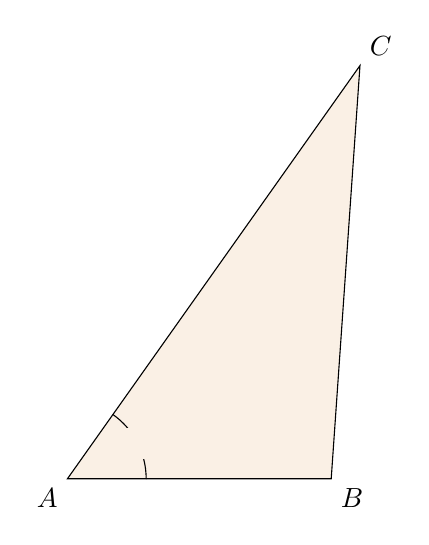
\begin{tikzpicture}[scale=\scale]

	\coordinate (A) at (0,0);
	\coordinate (B) at (3.35,0);
	\coordinate (C) at ($ (A) + (54.7:6.43) $);

	\filldraw[fill=Linen, draw=black] (A) -- (B) -- (C) --  cycle;
	
	\draw[below right] (B) node {$B$};
	\draw[below left] (A) node {$A$};
	\draw[above right] (C) node {$C$};

	\draw (1,0)  arc(0:54.7:1) node[xshift=2mm, fill=Linen, inner sep=2mm] at (24:1.1){$\qquad$};



\end{tikzpicture}

\end{frame}

%%%%%%%%%%%%%%%%%%%%%%%%%%%%%%%%%%%%%%%%%%%%%%%%%%%%%%%%%%%%%%%%%%%%%%%%%%%%%%%%%%%%%%%%%%%%%%%%%%%
\begin{frame}{Similar Triangles Exercises}
  \input{../pikz/01MathReview/simTrianglesQwizm}
\end{frame}

%%%%%%%%%%%%%%%%%%%%%%%%%%%%%%%%%%%%%%%%%%%%%%%%%%%%%%%%%%%%%%%%%%%%%%%%%%%%%%%%%%%%%%%%%%%%%%%%%%%
\begin{frame}{Similar Triangles and Trig Functions}
  \input{../pikz/01MathReview/simTriangles2Qwizm}
\end{frame}

%%%%%%%%%%%%%%%%%%%%%%%%%%%%%%%%%%%%%%%%%%%%%%%%%%%%%%%%%%%%%%%%%%%%%%%%%%%%%%%%%%%%%%%%%%%%%%%%%%%
\begin{frame}{Triangles and Trig Functions}
  \input{../pikz/01MathReview/TrianglesAndTrigQwizm}
\end{frame}


%%%%%%%%%%%%%%%%%%%%%%%%%%%%%%%%%%%%%%%%%%%%%%%%%%%%%%%%%%%%%%%%%%%%%%%%%%%%%%%%%%%%%%%%%%%%%%%%%%%
\section{Math Review}
%%%%%%%%%%%%%%%%%%%%%%%%%%%%%%%%%%%%%%%%%%%%%%%%%%%%%%%%%%%%%%%%%%%%%%%%%%%%%%%%%%%%%%%%%%%%%%%%%%%

\begin{frame}{Right Triangle}
  Note: $a, b$ and $c$ are shown after transition.
  \vspace{1cm}
  \input{../pikz/01MathReview/math01}
\end{frame}

%%%%%%%%%%%%%%%%%%%%%%%%%%%%%%%%%%%%%%%%%%%%%%%%%%%%%%%%%%%%%%%%%%%%%%%%%%%%%%%%%%%%%%%%%%%%%%%%%%%
\begin{frame}{Right Triangle Exercises}
  \resizebox{0.75\textwidth}{!}{%
  \input{../pikz/01MathReview/math04}
}
\end{frame}

%%%%%%%%%%%%%%%%%%%%%%%%%%%%%%%%%%%%%%%%%%%%%%%%%%%%%%%%%%%%%%%%%%%%%%%%%%%%%%%%%%%%%%%%%%%%%%%%%%%
\begin{frame}{Sine Rule Exercises}
  % !TEX root = ../../statikz2020/statikz2020.tex

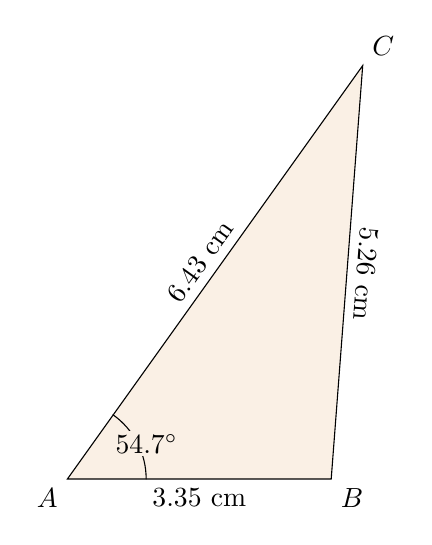
\begin{tikzpicture}[scale=\scale]

	\coordinate (A) at (0,0);
	\coordinate (B) at (3.35,0);
	\coordinate (C) at ($ (A) + (3.75,5.25) $);

	\filldraw[fill=Linen, draw=black] (A) -- node[sloped, above] {$6.43$ cm} (C) -- node[sloped, above, rotate=180]{$5.26$ cm}(B) -- node[below, sloped] {$3.35$ cm} cycle;
	
	\draw[below right] (B) node {$B$};
	\draw[below left] (A) node {$A$};
	\draw[above right] (C) node {$C$};

	\draw (1,0)  arc(0:54.7:1) node[fill=Linen, inner sep=0.4mm] at (24:1.1){$54.7^\circ$};



\end{tikzpicture}

\end{frame}

%%%%%%%%%%%%%%%%%%%%%%%%%%%%%%%%%%%%%%%%%%%%%%%%%%%%%%%%%%%%%%%%%%%%%%%%%%%%%%%%%%%%%%%%%%%%%%%%%%%
\begin{frame}{Similar Triangles Exercises}
  % !TEX root = ../../statikz2020/statikz2020.tex

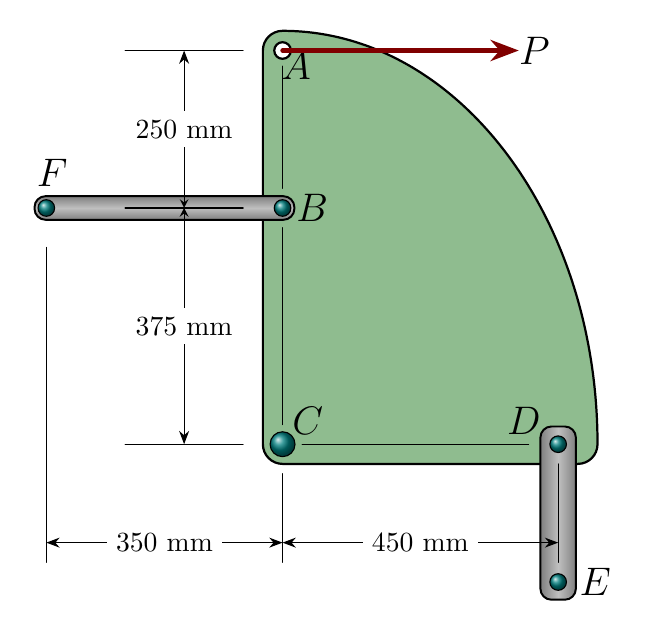
\begin{tikzpicture}

	\coordinate (C) at (0,0);
	\coordinate (B) at (0,3);
	\coordinate (A) at (0,5);
	\coordinate (D) at (3.5,0);
	\coordinate (E) at (3.5,-1.75);
    \coordinate (F) at (-3,3);

    \gettikzxy{(A)}{\ax}{\ay}
    \gettikzxy{(B)}{\bx}{\by}
    \gettikzxy{(C)}{\cx}{\cy}
    \gettikzxy{(D)}{\dx}{\dy}
    \gettikzxy{(E)}{\ex}{\ey}
    \gettikzxy{(F)}{\fx}{\fy}
    
    \PinnedConnection{C}{CadetBlue}{Black}{0.75}{0.25};
    \filldraw[fill=DarkSeaGreen, draw=black, thick] ($ (A)+(0,0.25)$) arc(90:180:0.25) --($ (C)+(-0.25,0) $)arc(180:270:0.25) -- ($ (D)+(0.25,-0.25)$)arc(270:360:0.25)arc[start angle=0, end angle=90, x radius=4cm, y radius=5.25cm];

    \PinnedConnection[-90]{F}{CadetBlue}{Black}{0.5}{0.25};
    
    \PinnedConnection{E}{CadetBlue}{Black}{0.5}{0.25};
    \Member{F}{B}{Grey}{Grey!50}{black}{0.3}{0.14}{0.25};
    \Member{D}{E}{Grey}{Grey!50}{black}{0.45}{0.14}{0.25};
    
    \filldraw[fill=white, draw=black, thick] (A) circle (3pt) node[xshift=1.75mm, yshift=-2mm]{\Large $A$};
    \shadedraw[ball color=Teal] (B) circle (3pt) node[right, xshift=0.5mm]{\Large $B$};
    \shadedraw[ball color=Teal] (C) circle (4.5pt) node[above right]{\Large $C$};
    \shadedraw[ball color=Teal] (D) circle (3pt) node[above left, xshift=-1mm]{\Large $D$};
    \shadedraw[ball color=Teal] (E) circle (3pt) node[right, xshift=1.5mm]{\Large $E$};
    \shadedraw[ball color=Teal] (F) circle (3pt) node[above, xshift=0.75mm, yshift=1.5mm]{\Large $F$};

    \draw ($ (F) + (0,-0.5) $) -- ($ (\fx, \ey+0.25cm)$);
    \draw ($ (D)+(0,-0.25)$) -- ($ (E)+(0,0.25) $);
    \draw ($ (C)+(0,-0.375)$) -- ($ (\cx, \ey+0.25cm) $);
    \draw ($ (A)+(0,-0.2)$) -- ($ (B)+(0,0.25) $);
    \draw ($ (B)+(0,-0.25)$) -- ($ (C)+(0,0.25) $);
    \draw ($ (A)+(-0.5,0)$) -- +(-1.5,0);
    \draw ($ (B)+(-0.5,0)$) -- +(-1.5,0);
    \draw ($ (C)+(-0.5,0)$) -- +(-1.5,0);
    \draw ($ (C)+(0.25,0)$) -- ($(D)+(-0.375,0)$);
    \draw [Stealth-stealth] ($ (A)+(-1.25,0)$) -- node[fill=white]{$250$ mm}($ (B)+(-1.25,0)$);
    \draw [stealth-Stealth] ($ (B)+(-1.25,0)$) -- node[fill=white]{$375$ mm}($ (C)+(-1.25,0)$);
    \draw [Stealth-Stealth] ($ (\fx, \ey+0.5cm)$) -- node[fill=white]{$350$ mm}($ (\cx, \ey+0.5cm)$);
    \draw [Stealth-Stealth] ($ (\cx, \ey+0.5cm)$) -- node[fill=white]{$450$ mm}($ (\ex, \ey+0.5cm)$);

    \draw [-Stealth, ultra thick, Maroon] (A)--+(3,0)node[black, xshift=2mm]{\Large $P$};

\end{tikzpicture}

\end{frame}

%%%%%%%%%%%%%%%%%%%%%%%%%%%%%%%%%%%%%%%%%%%%%%%%%%%%%%%%%%%%%%%%%%%%%%%%%%%%%%%%%%%%%%%%%%%%%%%%%%%
\begin{frame}{Similar Triangles and Trig Functions}
  % !TEX root = ../../statikz2020/statikz2020.tex

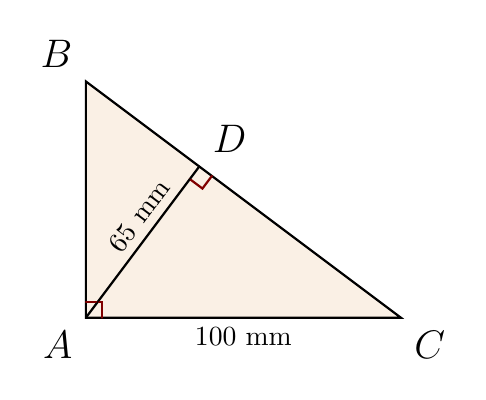
\begin{tikzpicture}

    \Large

	\coordinate (A) at (0,0);
	\coordinate (B) at (0,3);
	\coordinate (C) at (4,0);
	\coordinate (D) at ($(B)!0.36!(C)$);
	

    \gettikzxy{(A)}{\ax}{\ay}
    \gettikzxy{(B)}{\bx}{\by}
    \gettikzxy{(C)}{\cx}{\cy}
    \gettikzxy{(D)}{\dx}{\dy}
    
   \filldraw[fill=Linen, thick] (A)--(B)--(C)--cycle; 
   \draw[thick] (A)--(D); 
   \draw[Maroon, thick] (\ax+2mm,\ay)-- ++(0,0.2)-- ++(-0.2,0);
   \draw[Maroon, thick] ($(D)+(-36.9:0.2)$)-- ++(-126.9:0.2)-- ++(143.1:0.2);

   \node[below left] at (A){$A$};
   \node[above left] at (B){$B$};
   \node[below right] at (C){$C$};
   \node[above right] at (D){$D$};

   \normalsize

   \node[below] at ($(A)!0.5!(C)$){$100$ mm};
   \draw  (A) -- (D) node [sloped,pos=0.6,above] {$65$ mm};

\end{tikzpicture}

% \begin{tikzpicture}[domain=0:4]
% \draw[very thin,color=gray] (-0.1,-1.1) grid (3.9,3.9);
% \draw[->] (-0.2,0) -- (4.2,0) node[right] {$x$};
% \draw[->] (0,-1.2) -- (0,4.2) node[above] {$f(x)$};
% \draw[color=red] plot[id=x] function{x} node[right] {$f(x) =x$};
% \draw[color=blue] plot[id=sin] function{sin(x)} node[right] {$f(x) = \sin x$};
% \draw[color=orange] plot[id=exp] function{0.05*exp(x)} node[right] {$f(x) = \frac{1}{20} \mathrm e^x$};
% \end{tikzpicture}
\end{frame}

%%%%%%%%%%%%%%%%%%%%%%%%%%%%%%%%%%%%%%%%%%%%%%%%%%%%%%%%%%%%%%%%%%%%%%%%%%%%%%%%%%%%%%%%%%%%%%%%%%%
\begin{frame}{Triangles and Trig Functions}
  \input{../pikz/01MathReview/TrianglesAndTrig}
\end{frame}

%%%%%%%%%%%%%%%%%%%%%%%%%%%%%%%%%%%%%%%%%%%%%%%%%%%%%%%%%%%%%%%%%%%%%%%%%%%%%%%%%%%%%%%%%%%%%%%%%%%
\section{Forces \& Components}

%%%%%%%%%%%%%%%%%%%%%%%%%%%%%%%%%%%%%%%%%%%%%%%%%%%%%%%%%%%%%%%%%%%%%%%%%%%%%%%%%%%%%%%%%%%%%%%%%%%

\section{Frames \& Machines}

\begin{frame}{Frames \& Machines}
  complex frames will start here

  \ifnum\pdfshellescape=1
 Yes, enabled
\else
 No, disabled
\fi
\end{frame}

\end{document}
